\section{Catching Attackers at the university}

\begin{frame}{Network Recap}
    \begin{figure}
        \centering
        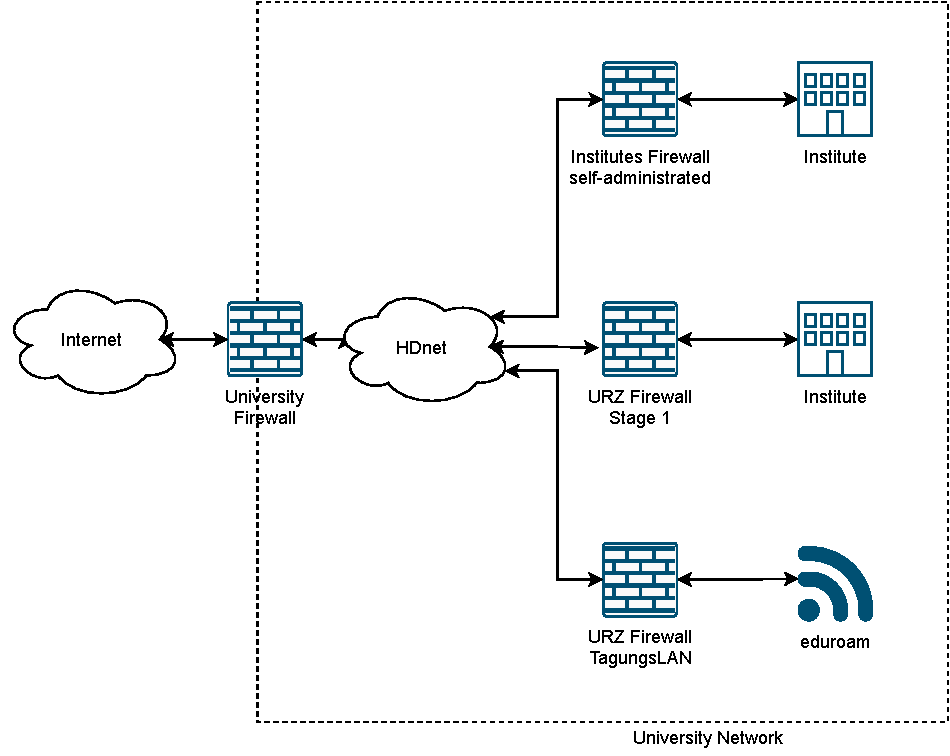
\includegraphics[width=0.8\columnwidth]{img/university-network.pdf}
        \caption[Draft of the university network]{
            Draft of the university network.
        }
    \end{figure}
\end{frame}

\begin{frame}{Introduction}
    Trying to answer the questions:
    \begin{itemize}
        \item Do attackers have access to restricted zones?
        \item Is it feasible to deploy attacks?
    \end{itemize}
\end{frame}

\begin{frame}{Concept}
    \begin{columns}[T]
        % Column 1
        \begin{column}{0.5\textwidth}
            \begin{block}{MADCAT}
                \textit{Mass Attack Detection Connection Acceptance Tools}
            \end{block}
            {\footnotesize
            \begin{itemize}
                \item Honeypot-like detection tool
                \item Logs every connection attempt
                \item Processes packets to retrieve exploitation
            \end{itemize}
            }
        \end{column}
        % Column 2
        \begin{column}{0.6\textwidth}
            \begin{itemize}
                \item Capturing attacks over 3 weeks
                \item Investigating \enquote{eduroam} and Stage 1 firewall
                \item Two local computers are connected to both networks
            \end{itemize}
        \end{column}
    \end{columns}
\end{frame}

\begin{frame}{Results}
    \begin{figure}
        \centering
        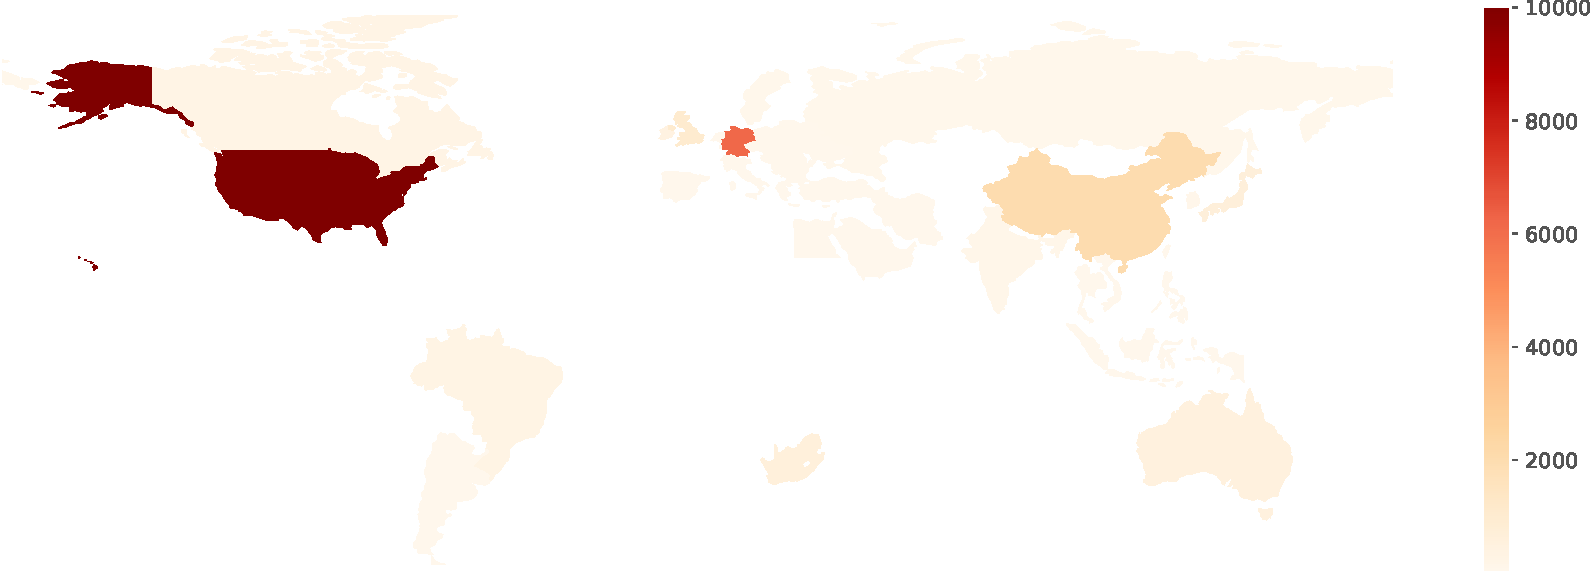
\includegraphics[width=\textwidth]{img/madcat-overview-map.pdf}
        \caption[Attack distribution of MADCAT]{
            Attack distribution of MADCAT.
        }
        \label{fig:madcat-attack-distribution}
    \end{figure}
\end{frame}

\begin{frame}{Results}
    \begin{figure}
        \centering
        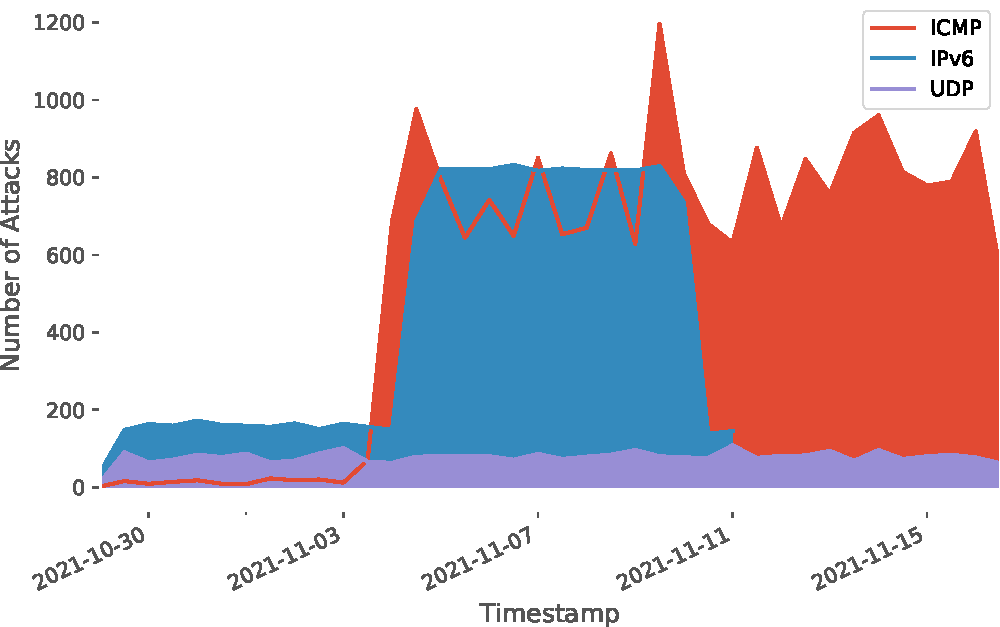
\includegraphics[width=\textwidth]{img/madcat-protocol-usage.pdf}
        \caption[Protocol distribution of MADCAT]{
            Protocol distribution of MADCAT.
        }
        \label{fig:madcat-protocols}
    \end{figure}
\end{frame}

\begin{frame}{Results}
    \begin{columns}
        % Column 1
        \begin{column}{0.4\textwidth}
            {\footnotesize
            \begin{itemize}
                \item Many RDP, SNMP, and TCP alerts
                \item Reflects day-to-day traffic
            \end{itemize}
            }
        \end{column}
        % Column 2
        \begin{column}{0.6\textwidth}
            \begin{figure}
                \centering
                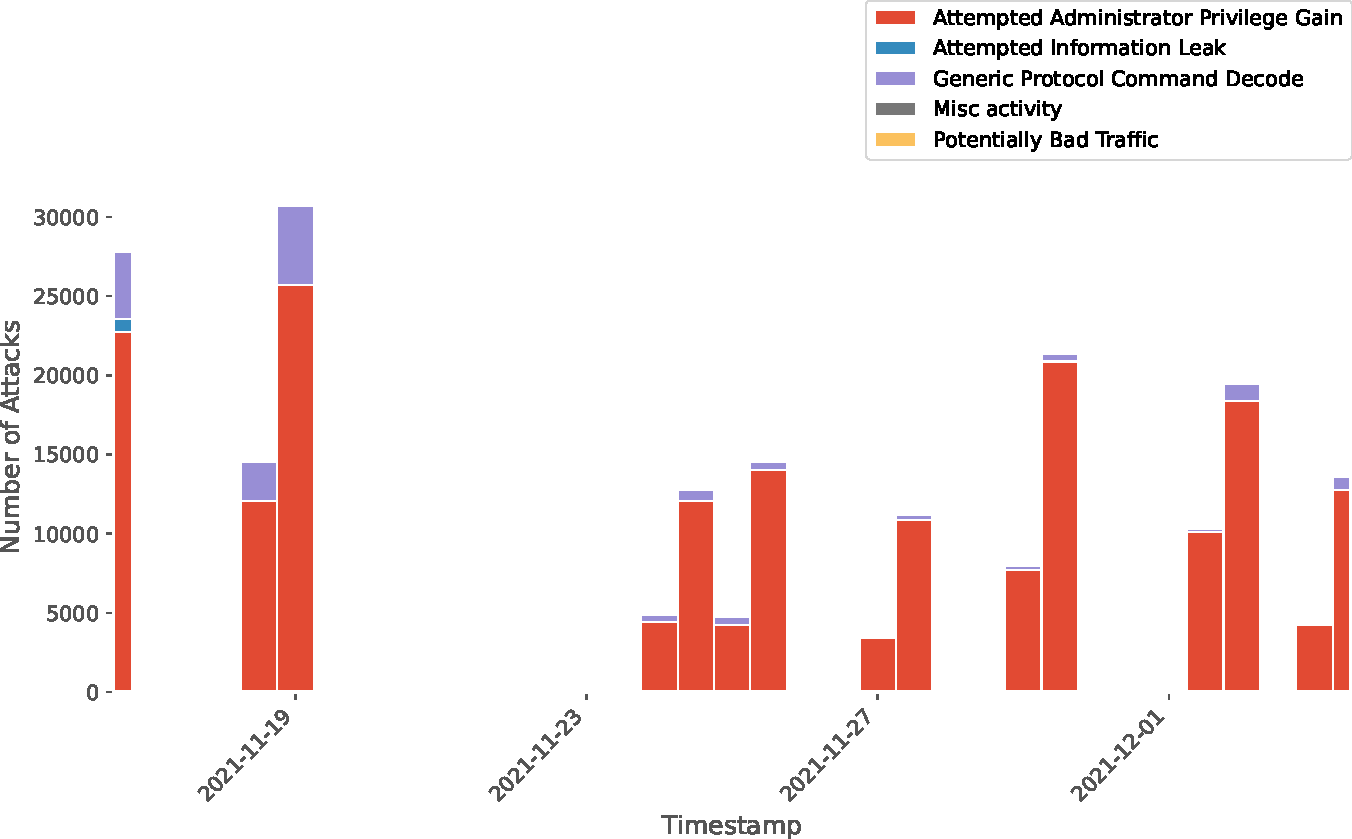
\includegraphics[width=\textwidth]{img/madcat-suricata-alerts.pdf}
                \caption[Suricata results]{
                    Suricata results.
                }
                \label{fig:suricata-distribution}
            \end{figure}
        \end{column}
    \end{columns}
\end{frame}

\begin{frame}{Summary}
    \begin{itemize}
        \item Identified the open port 113
        \begin{itemize}
            \item IDENT protocol
            \item Deployed various attacks
            \item Will be closed soon
        \end{itemize}
        \item \enquote{eduroam} works by design
        \begin{itemize}
            \item Users are encapsulated
        \end{itemize}
        \item Validates the stateless firewall
    \end{itemize}
\end{frame}